\documentclass[10pt,a4paper]{article}
\usepackage{qsl-template}

%%%%%%%%%% Title Section %%%%%%%%%%
\title{\bfseries Title of the work}

%%%%%%%%%% Author(s) %%%%%%%%%%
\AuthorsBlock
{% No empthy line here
  \Author{First Author}{1}\AuthorSep
  \Author{Second Author}{1,2}\AuthorLastSep
  \Author{Third Author}{2}
}
{% No empthy line here
  \Affil{1}{Affiliation One, Department, Institution, City, Country}
  \Affil{2}{Affiliation Two, Department, Institution, City, Country}
}
{corresponding.author@email.com}

\begin{document}

\maketitle


%%%%%%%%%% Abstract %%%%%%%%%%
\abstract{
Write your abstract here. The abstract should concisely describe the scientific motivation,
methods, main results, and relevance to quantum sensing and related physics topics.
(keep it max. 150 words)}


%%%%%%%%%% Body %%%%%%%%%%
\section*{Introduction and Background}

The total length of the document, including figures and references, must fit on\textbf{ two pages}.

You may include equations using the standard \LaTeX{} environment:

\begin{equation}
\mathrm{P}_{g/h} = \frac{1}{2}[1\pm T\cos{\gamma}],
\end{equation}

or inline such as $\omega_p = \omega_s+\omega_i$.

You can include a figure using the \verb|figure| environment and reference it with
\verb|\ref|, see Fig.~\ref{fig:example}. To cite a paper, add it to
\verb|references.bib| and use \verb|\cite|. 
Example citations: \cite{Lemos_2014, Einstein-Podolsky-Rosen}.

\begin{figure}[h]
    \centering
    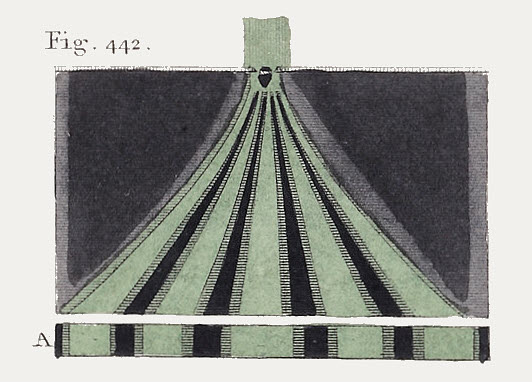
\includegraphics[width=0.75\textwidth]{figure.jpg}
    \caption{Example figure caption. Figures should be clear and readable.}
    \label{fig:example}
\end{figure}

The provided section names are suggestions only. Authors are free to rename, add (using \verb|\section*{}| command), or remove sections as appropriate.

\section*{Methods / Experiment}
Briefly describe the experimental setup, sensing protocol, or theoretical framework.

\section*{Results and Discussion}
Summarize the key results and their significance.

%%%%%%%%%% References %%%%%%%%%%
\bibliographystyle{unsrtnat}
\bibliography{references}

\end{document}
